\documentclass[doc]{apa}
\usepackage[utopia]{mathdesign}
\usepackage{graphicx,apacite,amsmath,rotating,verbatim,epsfig,subfigure}
\usepackage{dcolumn}
\usepackage{tikz}

\title{mcplR: An R-package for multiple cue learning models}
\author{Maarten Speekenbrink}
\affiliation{Department of Cognitive, Perceptual and Brain Sciences \\ University College London}

\abstract{
This paper introduces the mcplR package, an open source package for the R software environment to fit various multiple cue learning models. The package is introduced through the implementation of the Rescorla-Wagner model. A brief description of the other models currently implemented, such as the GCM and ALCOVE. 
}

\ifapamodedoc{%
\leftheader{Speekenbrink}
\rightheader{mcplR}
\acknowledgements{This research was supported by the ESRC Centre for Economic Learning and Social Evolution (ELSE).

Address correspondence to M. Speekenbrink, Department of Psychology, University College London, Gower Street, London WC1E 6BT, England, e-mail: \texttt{m.speekenbrink@ucl.ac.uk}}
}

\ifapamodejou{%
\leftheader{Speekenbrink}
\rightheader{mcplR}
\acknowledgements{Address correspondence to M. Speekenbrink, Division of Psychology and Language Sciences, University College London, 26 Bedford Way, London WC1H 0AP, England, e-mail: \texttt{m.speekenbrink@ucl.ac.uk}}
}

\ifapamodeman{%
	\note{
	\vspace{6em}
	\begin{flushleft}
    Dr. M. Speekenbrink\\
    Department of Psychology\\
    University College London \\
    Gower Street \\
    London WC1E 6BT \\ 
    England\\
    Tel:  +44 (0) 20 7679 7572 \\
    Fax: +44 (0) 20 7436 4276 \\
    E-mail: m.speekenbrink@ucl.ac.uk\\
   \end{flushleft}}}
{% else, i.e., in jou and doc mode 
\note{Draft of \today}}

\journal{To be submitted}

\renewcommand{\vec}[1]{\text{\bf{#1}}}
\newcommand{\mat}[1]{\text{\bf{#1}}}
\newcommand{\tr}{\text{tr}}
\newcommand{\logit}[1]{\log \left( \frac{#1}{1 - #1} \right)}
\newcommand{\logodds}[2]{\log \left( \frac{#1}{#2} \right)}
\newcommand{\slogit}[1]{\log( \tfrac{#1}{1 - #1})}
\newcommand{\mean}[1]{\overline{#1}}
\newcommand{\sign}{\text{sgn}}
\newcommand{\tif}{\text{ if }}

\newcommand{\greekv}[1]{\mbox{\boldmath$#1$}}
\newcommand{\greekm}[1]{\mbox{\boldmath$#1$}}
\newcommand{\thetab}{\mbox{\boldmath$\theta$}}
\newcommand{\betab}{\mbox{\boldmath$\beta$}}
\newcommand{\mub}{\mbox{\boldmath$\mu$}}
\newcommand{\Sigmab}{\mbox{\boldmath$\Sigma$}}
\newcommand{\sigmab}{\mbox{\boldmath$\sigma$}}
\newcommand{\MSE}{\text{MS}_e}
\newcommand{\diag}{\text{diag}}
\newcommand{\mtr}{^{\textsf{T}}}

\newcommand{\code}[1]{{\ttfamily{#1}}}
%\newcommand{\code}[1]{{\verb{#1}}}

\newcolumntype{d}[1]{D{.}{.}{#1}}

\begin{document}
\maketitle

In Multiple Cue Probability Learning (MCPL) tasks, the objective is to predict a criterion variable from a number of cues which are probabilistically related to the criterion. This is an ubiquitous task in daily life. For instance, a stockbroker predicts share price from market indicators, and a doctor diagnoses diseases from multiple symptoms. Understandably, MCPL has received much attention in (cognitive) psychology. When the criterion is a nominal variable, it is commonly referred to as (probabilistic) category learning. When the criterion is a metric variable, it is often described as function learning or Social Judgement. Over the years, a large number of formal models have been proposed to describe how people learn to perform MCPL tasks. We describe here an \code{R} package which implements a number of these. Although formal modelling of learning processes has become more mainstream, it is still . Fitting these models to data By designing this package, I hope that researchers will find it more easy to estimate these models in their research. Although the number of models implemented is still limited, we plan to add more in the future. Moreover, the package has been designed such that users can relatively easily add their own preferred models. 

In the remainder of this article, we will first describe the general structure of MCPL models, and then discuss their implementation in \code{mcplR}. Basic features of the package are introduced through the implementation of the Rescorla-Wagner model. After an overview of the other models and methods implemented in the package, we end by briefly illustrating how to specify a new model. 

\section{The general structure of MCPL models}

In MCPL tasks, the objective is to predict a criterion variable on the basis of a number of cues. On each trial $t = 1,\ldots,T$, cue values $\vec{x}_t = (x_{1t},\ldots,x_{mt})$ are presented, and the learner makes a prediction $R_t$ about the value of the criterion. After this, outcome feedback on the true value of the criterion, $Y_t$, is given. The learner is to use this outcome feedback to improve upon his or her predictions.

\begin{figure}
\centering
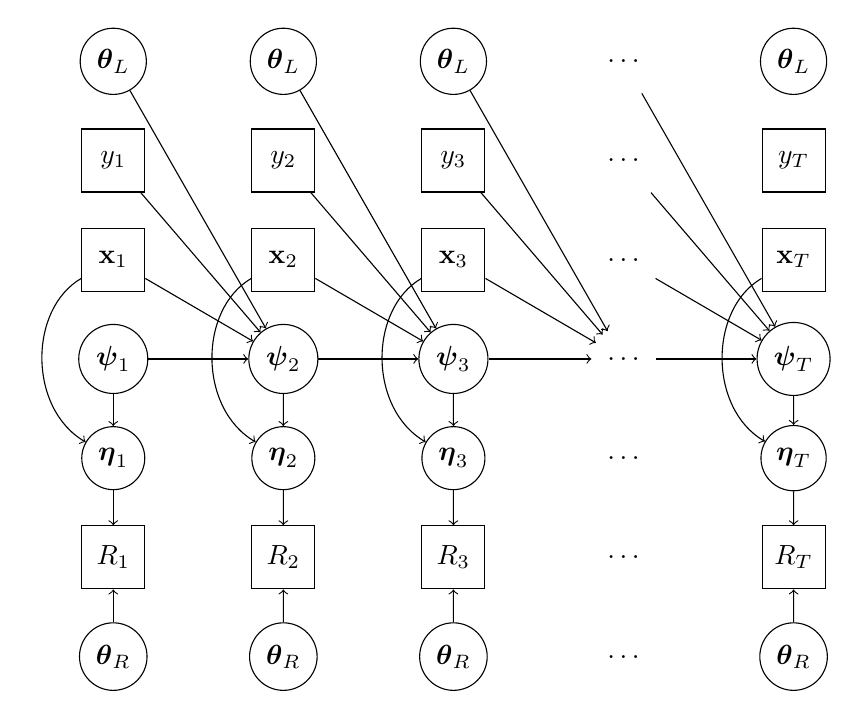
\begin{tikzpicture}[scale=.9]
		\begin{scope}[]{
			\pgfsetxvec{\pgfpoint{2.4cm}{0cm}}
			\pgfsetyvec{\pgfpoint{0cm}{1.4cm}}
			\tikzstyle{every node}=[minimum size=.8cm]


				\draw	node[draw,circle] (thetaR1) at (0,-2) {$\greekv{\theta}_R$};
				\draw node[draw,circle] (thetaR2) at (1,-2) {$\greekv{\theta}_R$};
			  \draw	node[draw,circle] (thetaR3) at (2,-2) {$\greekv{\theta}_R$};
				\draw	node (thetaRdots) at (3,-2) {$\ldots$};
				\draw	node[draw,circle] (thetaRT) at (4,-2)  {$\greekv{\theta}_R$};
				
				\draw	node[draw] (r1) at (0,-1) {$R_1$};
				\draw node[draw] (r2) at (1,-1) {$R_2$};
			  \draw	node[draw] (r3) at (2,-1) {$R_3$};
				\draw	node (rdots) at (3,-1) {$\ldots$};
				\draw	node[draw] (rT) at (4,-1)  {$R_T$};

				\draw	node[draw,circle] (eta1) at (0,0) {$\greekv{\eta}_1$};
				\draw node[draw,circle] (eta2) at (1,0) {$\greekv{\eta}_2$};
			  \draw	node[draw,circle] (eta3) at (2,0) {$\greekv{\eta}_3$};
				\draw	node (etadots) at (3,0) {$\ldots$};
				\draw	node[draw,circle] (etaT) at (4,0) {$\greekv{\eta}_T$};
								
				\draw node[circle,draw] (psi1) at (0,1) {${\greekv{\psi}}_1$};
				\draw node[circle,draw] (psi2) at (1,1) {${\greekv{\psi}}_2$};
				\draw	node[circle,draw] (psi3) at (2,1) {${\greekv{\psi}}_3$};
				\draw	node[circle] (psidots) at (3,1) {$\ldots$};
				\draw	node[circle,draw] (psiT) at (4,1) {${\greekv{\psi}}_T$};
							
				\draw node[draw] (x1) at (0,2) {$\vec{x}_1$};
				\draw node[draw] (x2) at (1,2) {$\vec{x}_2$};
				\draw	node[draw] (x3) at (2,2) {$\vec{x}_3$};
				\draw	node (xdots) at (3,2) {$\ldots$};
				\draw	node[draw] (xT) at (4,2) {$\vec{x}_T$};
				
				\draw node[draw] (y1) at (0,3) {$y_1$};
				\draw	node[draw] (y2) at (1,3) {$y_2$};
				\draw	node[draw] (y3) at (2,3) {$y_3$};
				\draw	node (ydots) at (3,3) {$\ldots$}; 
				\draw	node[draw] (yT) at (4,3) {$y_T$};

				\draw	node[draw,circle] (thetaL1) at (0,4) {$\greekv{\theta}_L$};
				\draw node[draw,circle] (thetaL2) at (1,4) {$\greekv{\theta}_L$};
			  \draw	node[draw,circle] (thetaL3) at (2,4) {$\greekv{\theta}_L$};
				\draw	node (thetaLdots) at (3,4) {$\ldots$};
				\draw	node[draw,circle] (thetaLT) at (4,4)  {$\greekv{\theta}_L$};
				
				\draw[->] (psi1) -- (eta1);
				\draw[->] (psi2) -- (eta2);
				\draw[->] (psi3) -- (eta3);
				\draw[->] (psiT) -- (etaT);
				
				\draw[->] (x1) .. controls (-.5,1.5) and (-.5,0.5) .. (eta1);
				\draw[->] (x2) .. controls (.5,1.5) and (.5,0.5) ..  (eta2);
				\draw[->] (x3) .. controls (1.5,1.5) and (1.5,0.5)  ..  (eta3);
				\draw[->] (xT) .. controls (3.5,1.5) and (3.5,0.5) ..  (etaT);
				
				\draw[->] (eta1) -- (r1);
				\draw[->] (eta2) -- (r2);
				\draw[->] (eta3) -- (r3);
				\draw[->] (etaT) -- (rT);				
				
				
				\draw[->] (thetaR1) -- (r1);
				\draw[->] (thetaR2) -- (r2);
				\draw[->] (thetaR3) -- (r3);
				\draw[->] (thetaRT) -- (rT);
				
				\draw[->] (psi1) -- (psi2);
				\draw[->] (psi2) -- (psi3);
				\draw[->] (psi3) -- (psidots);
				\draw[->] (psidots) -- (psiT);		
						
				\draw[->] (x1) -- (psi2);
				\draw[->] (x2) -- (psi3);
				\draw[->] (x3) -- (psidots);
				\draw[->] (xdots) -- (psiT);
							
				\draw[->] (y1) -- (psi2);
				\draw[->] (y2) -- (psi3);
				\draw[->] (y3) -- (psidots);
				\draw[->] (ydots) -- (psiT);
				
				\draw[->] (thetaL1) -- (psi2);
				\draw[->] (thetaL2) -- (psi3);
				\draw[->] (thetaL3) -- (psidots);
				\draw[->] (thetaLdots) -- (psiT);
				}
			\end{scope}

\end{tikzpicture}
\caption{Representation of an MCPL model. The learning model involves updating representations $\greekv{\psi}_{t+1}$ on the basis of $\vec{x}_t$ and $y_t$. Representations and cues are used to form a prediction $\greekv{\eta}_t$, which is the basis of responses $R_t$.}
\label{fig:mcplmodel}
\end{figure}

An MCPL model consists of a learning and response submodel. The learning model describes how a representation of the environment is updated as new data comes in. This representation is generally the conditional distribution $P(Y_t|\vec{x}_t,\greekv{\psi}_t)$, where $\greekv{\psi}_t$ is the (abstract) representation as learned by the model. The response model describes how this representation is used to form predictions of the environment. 

The learning model uses the feedback $y_t$ on trial $t$ to update its representation of the environment. 

A main feature of MCPL models is that responses $R_t$ are conditionally independent given $\greekv{\eta}_t$, i.e.
\begin{equation}
P(R_1,\ldots,R_T|\greekv{\eta}_1,\ldots,\greekv{\eta}_T,\greekv{\theta}_R) = \prod_{t=1}^T P(R_t|\greekv{\eta}_t,\greekv{\theta}_R)
\end{equation}
The predictions follow from the task representations $\psi_t$ and probe cue patterns $\vec{x}_t$, e.g.
\begin{equation}
\greekv{\eta}_t = f(\greekv{\psi}_t,\vec{x}_t).
\end{equation}

A graphical representation is given in Figure~\ref{fig:mcplmodel}. 

While the response model is always assumed a statistical model, in many cases the learning model is not. In many learning models, representations are updated as
\begin{equation}
\greekv{\psi}_{t+1} = g(\greekv{\psi}_t,\vec{x}_t,y_t,\greekv{\theta}_L),
\end{equation}
where $g$ is some (non-linear) deterministic function. For instance, the Rescorla-Wagner model \cite{Rescorla72} involves updating stimulus response associations $\greekv{\psi}_t$ in this form. As we will see later, the GCM is different, but still deterministic, in the sense that a particular set of paired cue and criterion values $(\vec{x}_{1:t},y_{1:t})$ and parameters $\greekv{\theta}_L$ always result in the same representation $\greekv{\psi}_t$. There are exceptions to this (such as Anderson's \citeyear{Anderson91} Rational Model of Categorization), but these are currently not implemented in \code{mcplR}. Note that determinism is not a requirement to implement learning models in \code{mcplR}. However, the default estimation relies on numerical optimization routines which will give inconsistent results if $\greekv{\psi}_{1:T}$ differs from iteration to iteration. Hence, for probabilistic learning models, a different estimation routine will have to be implemented.

\begin{equation}
\greekv{\eta}_t = h(\greekv{\psi}_t,\vec{x}_t)
\end{equation}

\section{Implementation in \code{mcplR}}

The mcplR package has an object-oriented design, using R's ``S4'' classes and methods. MCPL models are defined by the \code{McplModel} class. This class has two slots: one for a \code{LearningModel} and one for a \code{ResponseModel}. Both these derive from the same basic \code{McplBaseModel} class, and consist minimally of a (predictor) matrix $\mat{X}$, a (criterion) matrix $\mat{Y}$, and a parameter list $\greekv{\theta}$. For the learning model, the predictor matrix will typically contain the cues $\vec{x}_t$ and the criterion matrix the values of the criterion $y_t$, $t=1,\ldots,T$. For the response model, the predictor matrix will typically contain the values of $\greekv{\eta}_t$, and the response matrix the responses $r_t$. 

%At the heart of the \coded{mcplR} package is the class \code{McplModel}. An \code{McplModel} contains of two submodels, namely a \code{LearningModel} and a \code{ResponseModel}. Both these are derived from a general \code{McplBaseModel}, which contains a slot for a dependent variable ($y$), a slot for predictor variables ($x$), and a slot for a list with parameters. For a \code{LearningModel}, the criterion will usually be the dependent variable, and the cues the predictor variables. For a \code{ResponseModel}, the dependent variable will usually be the response variable, and the predictor variables (some function of) the predictions of the learning model. Both learning and response model can contain free variables.

In addition to class definitions, the \code{mcplR} package defines a number of methods which operate on these classes. The most important from the users viewpoint is probably the \code{fit} method, by which to obtain (ML) estimates of the model parameters $\greekv{\theta} = (\greekv{\theta}_L,\greekv{\theta}_R)$. By default, estimation relies on the the \code{optim} function of \code{R} to numerically minimize the negative log-likelihood of the model. If the \code{logLik} method is unavailable for the response model, least squares estimation will be attempted. Another important method is the \code{runm} method, which when applied to a learning model computes the representations $\greekv{\psi}_t$, and when applied to an MCPL model, computes both representations $\greekv{\psi}_t$ and $\greekv{\eta}_t$. 

In the following section, we will illustrate the various options with an example 

\section{Example: the Rescorla-Wagner model}

As an example, we will discuss how to fit a Rescorla-Wagner model. The Rescorla-Wagner model \cite{Rescorla72} is a well-known associative learning model. It describes the strengthening of associative links between unconditioned and conditioned stimuli over paired presentations. On a given trial, a number of conditioned stimuli are presented and associated with an unconditioned stimulus. From these paired presentations, a (human) animal learns to expect the unconditioned stimulus when encountering the conditioned stimulus, and as a result shows a conditioned response. The expectation is due to the formation of associative links between conditioned and unconditioned stimulus, resulting in a link between the conditioned stimulus and the conditioned response. 

From trial $t$ to $t+1$, the associative strength between a CS (cue) $X_j$ and US (criterion) $Y_k$ is updated as
\begin{equation}
\psi_{j,k}(t+1) = \begin{cases} \psi_{j,k}(t) + \alpha_j \beta_{k,1} [\lambda_k - \sum_j x_j(t) \psi_{i,k}(t)] \quad \text{when US $k$ is present at trial $t$} \\
\psi_{j,k}(t) + \alpha_j \beta_{k,2} [0 - \sum_j x_j(t) \psi_{i,k}(t)] \quad \text{when US $k$ is absent on trial $t$} \\
\end{cases}
\end{equation}
where $\lambda_k$ is the maximum level of associative strength of US $k$, $x_j(t)$ the value of the CS $j$ at trial $t$ (0 when CS $j$ is not present at $t$), $\alpha_j$ the salience of CS $j$, and $\beta_k$ the salience of the US $k$, which can be dependent on the presence or absence of $y_k(t)$.

%Let $\vec{y}_t = (y_k(t)$ be a variable with value 0 when US $k$ is absent on trial $t$, and $\lambda$ when US $k$ is present (note that this does not have to be a single value, e.g., US $k$ can be present in different magnitudes). Similarly, let 

Complete code for the example can be found in Figure~\ref{fig:R-W}. 


\begin{figure}
\begin{verbatim}
# load the mcplR package
library(mcplR)
# load the Weather Prediction Task example data
data(WPT)
# create a learning model
lMod <- RescorlaWagner(y ~ x1+x2+x3+x4,data=WPT,ntimes=c(200,200),remove.intercept=TRUE)
# show (default) parameters
getPars(lMod)
# create a response model
rMod <- RatioRuleResponse(r~1,data=WPT,ntimes=c(200,200))
# combine in an McplModel
mMod <- McplModel(lMod,rMod)
# estimate the free parameters
fMod <- fit(mMod)
# summary
summary(fMod)
# plot the associative weights
plot(fMod)
\end{verbatim}
\caption{Example code to construct and estimate a Rescorla-Wagner model with a ratio response rule.}
\label{fig:R-W} 
\end{figure}

\subsection{Creating a Rescorla-Wagner learning model}

A Rescorla-Wagner model can be created by calling the \code{RescorlaWagner()} function. The first argument of the function is a \code{formula} object describing the learning environment. The left hand side of the formula specifies the criterion (\code{y}) and the right hand side specifies the cues. Evaluation of the formulas in mcplR is similar to how formulas are evaluated in R's \code{lm()} and \code{glm()} function; thus, one can easily specify a model which also includes interactions between the cues. In the example in Figure~\ref{fig:R-W}, a simple model with four cues is constructed.  The \code{data} argument gives the name of the data frame that contains the values of the cues and criterion. In the example, the \code{WPT} dataset is used, which comes with \code{mcplR} and contains data from a control and amnesic participant in the study reported by \cite{Speekenbrink08}. The \code{ntimes} argument is used to indicate that the dataset contains data of multiple participants; it is a list with, for each participant in the data, the number of trials. The WPT data contains two participants, who each completed 200 learning trials. The \code{remove.intercept} argument is used to force removal of the intercept that is included in the design matrix (i.e., slot ``x'') by default. In the example, no parameter argument is given. As a result, default parameter values are used. By default, the model has a single $\alpha$ parameter, identical for each cue, initialized at $\alpha = 0.1$. All $\beta$ parameters are initialized to 1, while the associative strength of each cue is initialized at 1. We can view the parameter values by calling \code{getPars(lMod)}, which returns shows the contents the model's parameter list.  % For instance, for an event $y$ with two levels, and four cues $x_j$, we can use 
%\code{lMod <- RescorlaWagner(y \textasciitilde x1+x2+x3+x4,data=WPT,ntimes=c(200,200),remove.intercept=TRUE)}
%which will create a Rescorla-Wagner model with 
 
\subsection{Creating a response model}

The Rescorla-Wagner model is a learning model, in that it makes no direct claim as to how the associations are reflected in responses. By linking the learning model to a response model, we can investigate such claims. In mcplR, responses usually depend on $\eta$, which itself is a function of $\psi$ and cues $\vec{x}$. By default, $\eta$ is computed by the calling \code{predict()} on the learning model. For a Rescorla-Wagner model, this results in the summed associations between each level of $Y$ and the cues: % we can pass a function of the expectancies to the response model.  As responses will usually be dependent on the expectancies, we let 
\begin{equation}
\eta_k(t) = \sum_j \psi_{j,k} x_j
\label{eq:eta_RW}
\end{equation}
To link these values to responses, a common choice is the (exponentiated) ratio response rule:
\begin{equation}
P(R_t=k) = \frac{\exp ( \beta \eta_k(t))} { \sum_j \exp (\beta \eta_j(t)) }
\end{equation}
A ratio response rule can be created by calling the \code{RatioRuleResponse()} function. The first argument to this function is again a formula. In this case, only the left hand side specifying the response is used; the right hand side is ignored as the predictors are computed from the learning model by Equation~\ref{eq:eta_RW}. This is usually the case with response models, although a more general model which incorporates its own predictors (in addition to those provided by the learning model) can be used (this is done in \code{GlmResponse}, for instance). 

\subsection{Estimating the model parameters}

After creating a learning and response model, they can be combined into an \code{McplModel}. We can then estimate the learning and response model parameters simultaneously, by calling the \code{fit} method for the McplModel. By default, this will minimize the negative log-likelihood of the response model by using R's built-in optimization routine, defaulting to the Nelder-Mead simplex method.  


\section{Other models and functions currently implemented in \code{mcplR}}

The package contains implementations of a number of learning and response models. The models currently included are listed in Table~\ref{tab:other_models}. Some of the models are complete MCPL models. For instance, the Generalized Context Model (GCM)  while others 

\begin{table}
\begin{tabular}{lll} \hline
name & type & description \\ \hline
ALCOVE & MCPL model & \\
BLF & MCPL model & Bayesian Linear Filter \cite{Speekenbrink10} \\
GCM  & MCPL model & Generalized Context Model \cite{Nosofsky86} \\
gGCM & MCPL model & an (even) more general GCM  \cite{Speekenbrink10}, allowing a categorical or metric criterion, as well as temporal decay \\
GaussianResponse & response model & \\
GuassianMixtureResponse & response model & \\
GlmResponse & response model & Models responses as a Generalized Linear Model (GLM). Allows inclusion of covariates in addition to predictions from learning models. \\
RescorlaWagner & learning model & The Rescorla-Wagner model. \\
SLFN & learning model & Single Layer Feedforward Network \\ \hline
\end{tabular}
\end{table}


%\section{Useful methods and functions}

In addition to the \code{fit} method, there are default methods for model evaluation. In particular, standard model selection criteria, such as the AIC, BIC, and (pseudo-) $R^2$ are defined. In addition, many models have default plotting methods. For instance, calling \code{plot()}, where \code{tMod} is the one estimated in the example, we obtain the plot of Figure XXX. 

\section{Defining new models}

The ratio rule response model assumes that on each trial, a choice is made from the same set. However, associative learning experiments often use a design in which the choice set changes at different stages. To implement this, we can define a new response model which identifies between which options a choice is made. The full code is given in Appendix A. Here, we will briefly comment on the various steps in defining new classes and methods. 

The first step is to define a new class. As the model need a ratio rule model with varying choice sets, we let the \code{ChoiceSetResponse} class inherit from the \code{RatioRuleResponse} class. To be able to estimate the parameters of the model, the model minimally needs a \code{logLik} or \code{predict} method. For a completely new class, these won't be defined, but in this case the methods are inherited from the \code{RatioRuleResponse} class. 

While not strictly necessary, it is also convenient to define a constructor function to construct new members of the class (see Appendix A).

To define new learning models, the steps are essentially the same. However, there is generally no need to define \code{logLik} methods for learning models. Instead, learning models require \code{predict} methods, which are used to compute the values of $\eta_k(t)$ in the response model.


\section{Extending \code{mcplR}}

The \code{mcplR} package was designed with the objective of being relatively easily extendable. 

To add a new learning model, users must define a new class which inherits from the \code{LearningModel} class. Then, they should minimally define a \code{predict} method. Ideally, other methods, such as \code{logLik}, would also be defined, but these are not required to estimate the models parameters when incorporated into an \code{McplModel}. In many cases, users can rely on the default methods.

To add a response model, users must again define a new class which inherits from the \code{ResponseModel} class. In addition, they must also minimally define either the \code{logLik} method or the \code{predict} method. If only the latter is defined, the model parameters will be estimated by OLS, while if the former is defined, ML estimates can be obtained. 



\section{Conclusion}

We introduced the \code{mcplR} extension package for the R language and framework. The package provides a flexible framework to specify and estimate learning models. A number of commonly used models is included. 

In the future versions of \code{mcplR}, we plan to:
\begin{itemize}
\item incorporate other learning and response models
\item allow more general parameter constraints
\end{itemize}

\bibliography{bibliography}

\appendix

\section{Code to implement a \code{ChoiceSetResponse} model}

\begin{verbatim}

# define the class to extend RatioRuleResponse models
setClass("ChoiceSetResponse",
  contains="RatioRuleResponse",
  representation(
    choiceset = "matrix"
  )
)

# Most RatioRuleResponse methods can be used directly
# apart from the predict method ...
  
setMethod("predict",signature(object="ChoiceSetResponse"),
  function(object,...) {
    out <- object@transformation(object,...)
    out <- (out*object@choiceset)/rowSums(out*object@choiceset)
    if(!is.matrix(out)) out <- matrix(out,ncol=1)
    out
  }
)

# Define a constructor function

ChoiceSetResponse <- function(formula,choiceset,parameters=list(beta=1),
  transformation=c("exponential","none"),data,ntimes=NULL,replicate=TRUE,fixed,
  parStruct,subset) {

    # construct a RatioRuleResponse model to extend
    call <- match.call()
    call[[1]] <- as.name("RatioRuleResponse")
    md <- eval(call,parent.frame())
  
    # check if choiceset is valid
    if(!all(dim(object@y) == dim(choiceset))) {
     stop("choiceset must have samedimension as response matrix")
    }
    if(!all(unique(choiceset) %in% c(0,1))) {
     stop("choiceset must be an indicator matrix")
    }
    
    # construct a ChoiceSetResponse
    mod <- new("ChoiceSetResponse",
      x = md@x,
      y = md@y,
      parStruct=md@parStruct,
      nTimes=md@nTimes,
      transformation=md@transformation,
      choiceset=choiceset)
    mod <- runm(mod)
    mod            
}
\end{verbatim}

\end{document}

A GCM can be specified by the function \code{GCM(formula,data,parameters,...)}. This function creates an object of the class \code{GCM}, extending the \code{LearningModel} class. To estimate the model's parameters, we can call the \code{estimate(object,...)} method. This will result in estimates which maximize the likelihood of the criterion. However, we will often want to use the \code{GCM} model as part of an \code{McplModel}. The ``classical'' GCM \cite{Nosofsky86} uses
\begin{equation}
P(R=j) = \frac{S_j^\lambda}{\sum_{k=1}^K S_k^\lambda}
\end{equation}
which is implemented in \code{mcplR} by a \code{RatioRuleResponse} model. This can be created by calling \code{RatioRuleResponse(formula,...)}, where only the left-hand side of the \code{formula} is evaluated. Starting values for the parameters can be given by an optional \code{parameters} argument. If this argument is not given, default starting values will be used (in this case, $\lambda=1$).

\subsection{Learning Model}

The GCM is different from other learning models in that it does not involve . Rather, learning consists of storing exemplars $(\vec{x}_t,y_t)$. To keep within the present framework, we can take the representation $\greekv{\psi}_t(\vec{x})$ to be a function 

\subsection{Response Model}

The GCM assumes that responses follow Luce's ratio rule, such that
\begin{equation}
P(R = j|\vec{x}) = \frac{V_j^\lambda}{\sum_k V_k^\lambda}
\end{equation}
Note that that the value of $V_j$ is given by the learning model. The response model thus contains a single free parameter, $\lambda$.

\subsection{Estimation}

The freely estimable parameters of the GCM are collected in the parameter vector $\greekv{\theta} = (,\lambda)$. Maximum likelihood estimates of these parameters are obtained by numerical maximisation of the likelihood $P(R|\greekv{\theta})$, specified in the response model. By default, numerical optimization is done by the Nelder-Mead simplex algorithm as implemented in the \code{optim} function of \code{R}. Other estimation procedures can be specified at the level of specific classes deriving from \code{McplModel}. There is also a switch to allow conditional maximisation of the response model parameters. In some cases, maximum likelihood estimates of the response model parameters can be derived in closed form (conditional on the learning model parameters), so that conditional estimation can decrease the computation required.

By default, the latter values are computed by calling the \code{predict} method on the learning model, with argument \code{type="link"} (this terminology is borrowed from Generalized Linear Models and indicates that the prediction is not on the scale of the criterion $y_t$, but on the scale of the internal representation $\greekv{\eta}_t$). The \code{lFr} method then passes this prediction on to the \code{x} slot of the response model. Usually, the \code{runm} method need not perform any further action on a response model\footnote{To save unneccesary computions, the \code{has.runm} method is called to check whether the \code{runm} method performs any computation. By default, this method returns FALSE.}.

The mechanics of the fit method are as follows:
\begin{enumerate}
\item Call \code{runm} method on the MCPL model:
\begin{enumerate}
\item Call \code{runm} on the learning model to compute $\greekv{\psi}_t$
\item Call the \code{lFr} method on the MCPL model. By default, this method calls the \code{predict(...,type="link")} method on the learning model, and copies the result to the \code{x} slot of the response model
\item If required, call the \code{runm} method on the response model to compute $\greekv{\eta}_t$
\item If required, call the \code{rFl} method on the MCPL model to pass the result back to the learning model
\end{enumerate}
\item Call the \code{logLik} method on the MCPL model to compute the negative log likelihood (of the responses)
\end{enumerate}
Starting with initial parameters, the optim routine loops through these steps until a (local) minimum in the negative log-likelihood is found. Users should be warned that there may multiple local minima, and it is good practice to try a number of different starting values to increase the chance of finding the global minimum.



\subsection{Learning models}

\subsection{Single Layer Feedforward Network (SLFN)}

A single layer feedforward network \cite<SLFN,>{Bishop95} is an artificial neural network model with one input layer, one output layer, and no hidden units. The connection weights are trained by the delta (or LMS) rule. This model can implement a (restricted) version of the Rescorla-Wagner model \cite{Gluck88,Speekenbrink08}, or be used as simple models of function learning \cite{Speekenbrink10}. 

%Associative learning models such as the Rescorla-Wagner model can be implemented by an artificial neural network \cite{Gluck88} with one input layer and one output layer. These networks are also known as Single Layer Feedforward Network models \cite<SLFN,>{Bishop95}. The SLFN model offers a general implementation which learns the connection weights by the delta (or LMS) rule. 
%\begin{equation}
%\vec{w}_{t+1}^{(i,j)} = \vec{w}_{t}^{(i,j)} + \frac{\greekv{\eta}^{(i,j)}}{t^{\alpha^{(i,j)}}} \delta^{(i,j)}_t + \greekv{\beta}^{(i,j)}(\vec{w}_t^{(i,j)} - \vec{w}^{(i,j)}_{t-1})
%\end{equation}
%where $\delta^{(i,j)}_t$ is the gradient of the activation function, e.g.
%\begin{equation}
%\delta^{(i,j)}_t = (Y_{t}^{(j)} - \vec{w}_t^{(i,j)} \vec{x}_t^{(i)}) \vec{x}_t^{(i)}
%\end{equation}
%if the activation function is linear. The parameters $\alpha$, $\beta$, and $\eta$ are usually scalars, so that they are identical for all cues $i$ and criterion values $j$. But they can optionally be vectors or matrices. 
An SLFN learning model can be created through the function \code{SLFN(formula,data,...)}. The output nodes can be linear or logistic. 

\subsection{Generalized Context Model (GCM)}

The Generalized Context Model \cite<GCM,>{Nosofsky86}. 

GCM learning model can be created by the function \code{GCM(formula,data,...)}. This will create a default GCM model, with a city-block distance function and an exponential similarity gradient and a Ratio Rule response. The distance function can be changed to an euclidian or general Minkowski distance function by the option \code{distance=``euclidian''} or \code{distance=``minkowksi''}, respectively. An arbitrary function can also be used by using a function for the distance option. Similarly, the similarity gradient can be changed through the option \code{similarity=``gaussian''}. In addition, the version of the GCM allows the specification of a decay function \cite{Speekenbrink10}. By default, this is set to uniform, but other options are a power and exponential function.
 
\subsection{ALCOVE}

ALCOVE \cite{Kruschke92}.


\begin{table}
\caption{Selected methods and functions in the mcplR package}
\begin{tabular}{lll} \hline
name & description & example call \\ \hline
\code{plot} & default plots of mcpl models & \code{plot(mod)} \\
\code{simulate} & simulate responses from a \code{ResponseModel} (or the response part of an \code{McplModel}) & \code{simulate(mod)} \\
\hline
\end{tabular}
\end{table}
 
